% Introduction

% Main chapter title
\chapter{Introduction} 
% Change X to a consecutive number; for referencing this chapter elsewhere, use \ref{ChapterX}
\label{Chapter1} 
% This is for the header on each page
\lhead{Chapter 1. \emph{Introduction}}


\section{Motivation }
The error performance of the low density parity check  codes approach to Shannon limit, which make low density parity check code the best known codes. An active research is going on to implement the low density parity check decoder for storage devices to achieve the bit error rate of the order of $10^{-16}$. Thus, to make a low density parity check  decoder with a optimum cost and performance trade off is a challenging task.

\section{Organisation of the Report }

In chapter 1, we have discussed the basics of error correction in a communication channel. In chapter 2, we have discussed Min Sum decoding algorithm in detail. In chapter 3, we have shown the results of the C level implementation of Min Sum decoding algorithm. In chapter 4, we have discussed the concept and procedure to partition a parity check matrix. Level of parallelism is taken as a metric and results are plotted and discussed. In chapter 5, we have deployed partitioning in the matrix and modified the decoding algorithm to parallelise the hardware. In chapter 6, the conversion of the algorithms from C to VHDL is discussed along with results of the implementation of the algorithm on FPGA.
\section{Basics of Error Correction }
  
The goal of communication is to transmit a message and receive it correctly even after noisy transmission through the channel. This is achieved by introducing redundancy in the message at the transmitter side, called as encoding of message. The encoded message is called codeword. Then codeword is then transmitted through the noisy channel, which alters the codeword. By some error correcting algorithm the message is extracted back at receiver side, called decoding of the codeword. Thus, the error free transmission takes place by applying error correcting codes in communication system.\\
We have a k bit long message. To encode it we introduce m redundant bits (called parity bits) to form an $n(=m+k)$ bit long codeword. This category of codes are called (n,k) block codes. 

\subsection{Parity Check Matrix}

The codeword must satisfy a group of conditions to ensure error free transmission or to indicate the error has taken place. If error occurs, the error can be corrected by applying some algorithm on those group of conditions . The group of conditions are called parity check equations.The matrix form of the condition is called parity check matrix. \\
Example\cite{9}: If a code block $y=[b_1\, b_2\,b_3\, b_4\, b_5\, b_6]$ has to satisfy following parity check equations. 
\begin{align}
b_1 \oplus b_2 \oplus b_4 =0 \\
 b_2 \oplus b_3 \oplus b_5 =0 \\
b_1 \oplus b_2 \oplus b_3 \oplus b_6 =0 
\end{align}  
Then it's parity check matrix is as follows:
\begin{align}
 H= \left[ \begin{array}{cccccc}
1 & 1 & 0 & 1 & 0 & 0\\
0 & 1 & 1 & 0 & 1 & 0\\
1 & 0 & 0 & 0 & 1 & 1\\
0 & 0 & 1 & 1 & 0 & 1  
\end{array} \right]  
\end{align} 
s.t. $Hy^T=0$.

\subsection{Encoding of Message}
We can rewrite the above equations (1),(2),(3) as:
\begin{align}
b_4 = b_1 \oplus b_2 \\
b_5 = b_2 \oplus b_3 \\
b_6 = b_1 \oplus b_2 \oplus b_3  
\end{align}  
We can find parity check bits $b_4,b_5,b_6$ by message bits $b_1,b_2,b_3$.
Thus we can encode message bits to find codeword. \\
Encoding is preferably done in matrix form, by manipulating parity check matrix to find a generator matrix.
If parity check matrix can be written in the form
$H = [A, I_{n- k} ]$,
where A is an $(n-k)$xk binary matrix and $I_{n-k}$ is the identity matrix of order
$(n-k)$. The generator matrix is then
$G = [I_k , A^T ]$.
s.t $GH^T = 0$. \\
\begin{align}
[b_1 b_2 ... b_6]=[b_1 b_2 b_3] \left[ \begin{array}{cccccc}
1 & 0 & 0 & 1 & 0 & 1\\
0 & 1 & 0 & 1 & 1 & 1\\
0 & 0 & 1 & 0 & 1 & 1  
\end{array} \right]
\end{align}
 

Thus, if m is message block containing message bits $[b_1 b_2 b_3]$, then codeword can be generated as $y=mG$.

\subsection{Transmission of the Code Block}
The code block is then transferred through a noisy communication channel that corrupts the code block. According to the behaviour of the noise that is added to the code block, various models of communication channels exists. 
\subsubsection{Binary Symmetric Channel}
 As the name suggests the channel is binary, it has two input symbols and two output symbols. The channel is symmetric because the probability of receiving 0 when 1 was send is same as probability of receiving 1 when 0 was sent. The error probability is also called cross over probability. The transition probability diagram is shown in figure \ref{bsc}
 \begin{figure}[h]
\centering
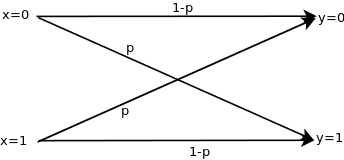
\includegraphics[height=6cm,width=12cm]{bsc}
\caption[Transition probability diagram of Binary Symmetric Channel]{Binary Symmetric Channel}
\label{bsc}
\end{figure}
The cross over probability is denoted as p.
\begin{align} p(y=0|x=1) = p(y=1|x=0) = p  \end{align}
\begin{align} p(y=1|x=1) = p(y=0|x=0) = 1-p  \end{align}
\subsubsection{AWGN (A White Gaussian Noise Channel)}
If a signal in a digital system is represented a continuous random variable as,
\begin{align} Y = X + Z \end{align}
where X is the digital information carrier and Z is the noise component then we can define a Gaussian channel that has input X and output Y, with noise as a Gaussian random variable Z. \\
The pdf of a Gaussian random variable is expressed as follows: \\
\begin{align} f_y(x) = \dfrac{1}{\sqrt{2\pi\sigma^{2}}} \exp{\dfrac{-(x-m)^2}{2\sigma^2}}
 \end{align} 
where m is mean and sigma is standard deviation of the random variable Z.
\subsection{Error Detection \& Correction}

If the codeword gets corrupted in the transmission then all the parity check equations will not get satisfied. Thus, we will get $Hy^T\neq0$. The non-zero vector is called syndrome. That shows that received message is corrupted. But there is a certain limit to the number of bits upto that error can be detected and corrected.
The limit is represented in term of hamming distance. Hamming distance between two codes is number of flipped bits between them. If $d_{min}$ is minimum distance between codes then maximum number of bits upto which error can be correctly detected is $d_{min}-1$ and maximum number of bits upto which error can be corrected is
(t) = $[\frac{d_{min}-1}{2}]$
where [] denotes greatest integer function.\\
More the number of redundant bits, more is the hamming distance. Thus, more error bits can be detected and corrected but the code rate is reduced. The correction is done by directly taking the received vector and comparing it to all the codewords and correcting it to the codeword having minimum distance to it. This is called maximum likelihood decoding. But if n is larger then this task becomes complex. LDPC maximum likelihood decoding, bit flipping decoding are other decoding schemes which reduce complexity of this task.









